%%%%%%%%%%%%%%%%%%%%%%%
%
%   Question 5
%
%%%%%%%%%%%%%%%%%%%%%%%

\noindent
{\textsc{\underline{Question 5 sur les graphes(\textbf{20} points)}}}\\

A tout mot $w= w_0, w_1, \ldots, w_n-1$ sur un alphabet fini $A$ on associe le \emph{graphe des mots} de longueur $k$, not\'e $G_k = (S_k, E_k)$ construit r\'ecursivement de la mani\`ere suivante:\medskip 
\begin{itemize}
\item[1.] $S_k =  \{w[0..(k-1)]\}; E_k = \{ \}$; % Sofiane : E_k = {w[k-1..,k]} non ? Car dans l'exemple les arcs ne portent qu'une seule lettre. 
\item[2.] Pour $ i = 0,1,2, n - k-1 $,  et\smallskip
\begin{itemize}  
  \item[-] $E_k = E_k \cup \{w[i .. (i+ k)]\}$; 
  \item[-] $S_k = S_k \cup \{w[(i+1) ..  (i+ k)]\}$ .
\end{itemize}
\medskip
\end{itemize}
Par exemple, consid\'erons le mot $w= bbaababaababba$ sur l'alphabet $A =\{a,b\}$. Son graphe  $G_3(w)$ est le graphe orienté $G$ suivant~:
\vspace{-.75cm}
\begin{center}
    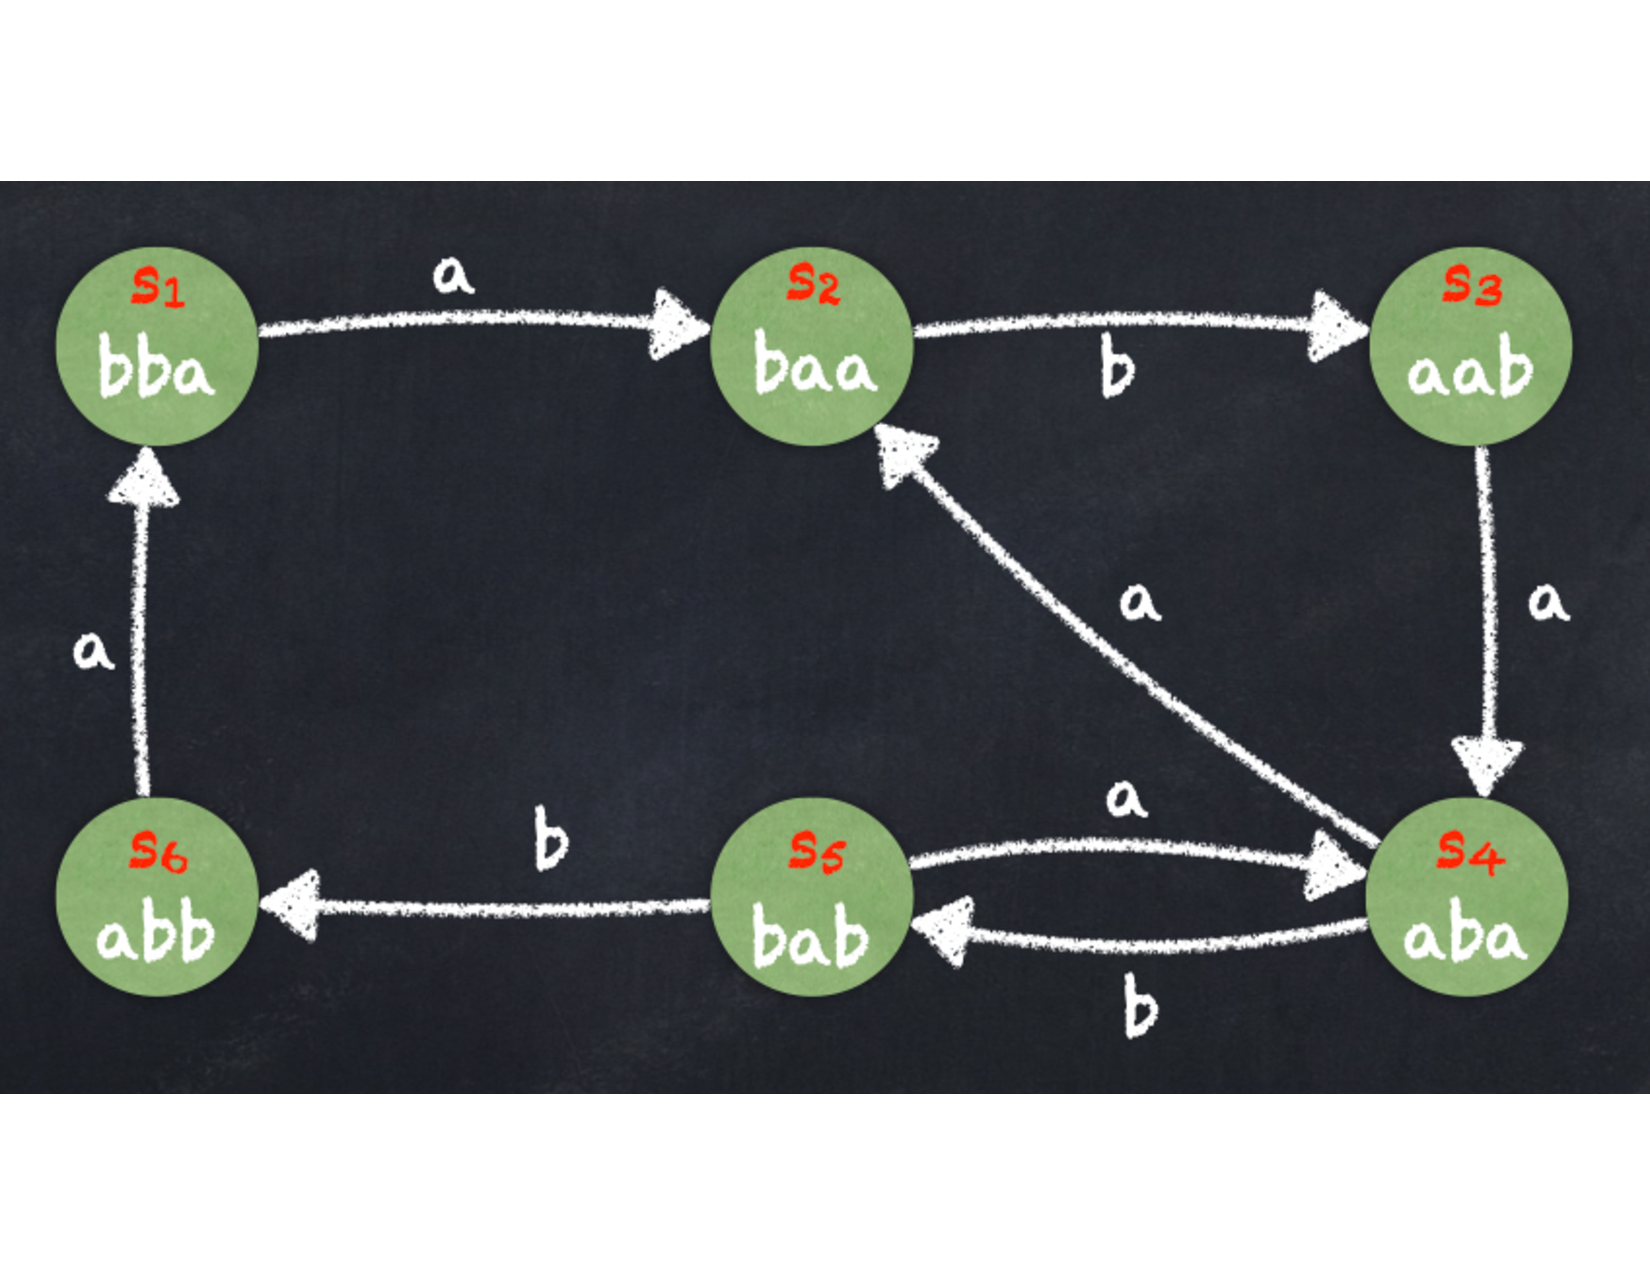
\includegraphics[width=3.5 in]{Figures/Graphe2.pdf} 
\end{center}
\vspace{-.75cm}
o\`u  le premier sommet  $s_1$ est  \'etiquet\'e par $w[0..2]=bba$, le deuxi\`eme  $s_2$ est \'etiquet\'e par $w[1..3]=baa$ et l' arc 
$e_1$ allant de $s_1$ \`a $s_2$, est étiqueté par $w[0..3] = bba.a$.
Cependant nous n'avons  mis que la lettre $a$ (par économie), car le début $bba$ est déjà écrit dans le sommet $s_1$.

\begin{enumerate}[\rm 1)]
\item\bareme{2} Donner sa repr\'esentation sous forme de liste d'adjacence. 
%%%%%%%%%%%%%%%%%%%%%%%%%%%%%%% 
% Solution                    %
%%%%%%%%%%%%%%%%%%%%%%%%%%%%%%%
\begin{framed}

RÉPONSE:\\
$s_1 \xrightarrow{}s_2$\\
$s_2 \xrightarrow{}s_3$\\
$s_3 \xrightarrow{}s_4$\\
$s_4 \xrightarrow{}s_2 + s_5$\\
$s_5 \xrightarrow{}s_4 + s_6$\\
$s_6 \xrightarrow{}s_1$\\

\end{framed}
%%%%%%%%%%%%%%%%%%%%%%%%%%%%%%%
\item \bareme{5} Donner sa repr\'esentation sous forme de matrice :\\
 \quad a) d'adjacence \'etiquet\'ee $L_G$, et non-\'etiquet\'ee $M_G$;  \\
 \quad b) d'incidence. 

%%%%%%%%%%%%%%%%%%%%%%%%%%%%%%% 
% Solution                    %
%%%%%%%%%%%%%%%%%%%%%%%%%%%%%%%
\begin{framed}
a) la matrice d'adjacence \'etiquet\'ee et non-\'etiquet\'ee sont 
\[ L_G= 
 \begin{bmatrix}
 0&a &0&0&0&0\\
 0&0 &b&0&0&0\\
 0&0 &0&a&0&0\\
 0&a &0&0&b&0\\
 0&0 &0&a&0&b\\
 a&0 &0&0&0&0\\
\end{bmatrix}
\quad M_G= 
\begin{bmatrix}
 0&1 &0&0&0&0\\
 0&0 &1&0&0&0\\
 0&0 &0&1&0&0\\
 0&1 &0&0&1&0\\
 0&0 &0&1&0&1\\
 1&0 &0&0&0&0\\
\end{bmatrix}
\]

b) La matrice d'incidence est donn\'ee par : \\
A partir des dennées de l'enoncé, j'ai trouvé la correspondance de $e_1$, $e_2$, ...:\\
$e_1 \Longleftrightarrow s_1 \Longrightarrow s_2$\\
$e_2 \Longleftrightarrow s_2 \Longrightarrow s_3$\\
$e_3 \Longleftrightarrow s_3 \Longrightarrow s_4$\\
$e_4 \Longleftrightarrow s_4 \Longrightarrow s_5$\\
$e_5 \Longleftrightarrow s_5 \Longrightarrow s_4$\\
$e_6 \Longleftrightarrow s_4 \Longrightarrow s_2$\\
$e_7 \Longleftrightarrow s_5 \Longrightarrow s_6$\\
$e_8 \Longleftrightarrow s_6 \Longrightarrow s_1$
\setcounter{MaxMatrixCols}{20}
\[
\begin{matrix}
 &\vline&e_1 &e_2 &e_3 &e_4 &e_5&e_6&e_7 &e_8 \\
\hline
s_1&\vline&1&0&0    &0  &0 & 0&0&-1  \\
s_2&\vline&-1&1&0    &0  &0 & -1&0&0  \\
s_3&\vline&0&-1&1    &0  &0 & 0&0&0  \\
s_4&\vline&0&0&-1    &1  &-1 & 1&0&0  \\
s_5&\vline&0&0&0    &-1  &1 & 0&1&0  \\
s_6&\vline&0&0&0    &0  &0 & 0&-1&1  \\
\end{matrix}
\]



\end{framed}
%%%%%%%%%%%%%%%%%%%%%%%%%%%%%%%

\item\bareme{4}  Donner pour chaque sommet, les degr\'es intérieur et extérieur.
%%%%%%%%%%%%%%%%%%%%%%%%%%%%%%% 
% Solution                    %
%%%%%%%%%%%%%%%%%%%%%%%%%%%%%%%
\begin{framed}

\[
\begin{matrix}
 &\vline&s_1 &s_2 &s_3 &s_4 &s_5&s_6\\
\hline
d^+&\vline&1 &1 &1&2 &2& 1\\
d^-&\vline&1 &2 &1&2 &1& 1\\
\end{matrix}
\]

\end{framed}
%%%%%%%%%%%%%%%%%%%%%%%%%%%%%%%
\item\bareme{4}  Quel est le nombre de chemins distincts de longueur $4$ dans $G$~? 
%%%%%%%%%%%%%%%%%%%%%%%%%%%%%%% 
% Solution                    %
%%%%%%%%%%%%%%%%%%%%%%%%%%%%%%%
\begin{framed}

RÉPONSE:Le nombre de chemins distincts de longueur 4 dans G sont :\\ \\ \\ \\
\[ 
\quad (Nb_G)^4= 
\begin{bmatrix}
 0&1 &0&0&1&0\\
 0&0 &1&1&0&1\\
 1&1 &0&1&1&0\\
 0&2 &1&1&1&1\\
 1&1 &1&1&1&0\\
 0&0 &0&1&0&0\\
\end{bmatrix}
\]
$(Nb_G)^4=21$\\
Donc on a 21 chemins distincts de longueur 4 dans G.
\end{framed}
%%%%%%%%%%%%%%%%%%%%%%%%%%%%%%%
\item\bareme{5}  Quelle est la longueur des chemins les plus courts entre toute paire de sommets distincts~?
%%%%%%%%%%%%%%%%%%%%%%%%%%%%%%% 
% Solution                    %
%%%%%%%%%%%%%%%%%%%%%%%%%%%%%%%
\begin{framed}

RÉPONSE: \\
Pour trouver la longueur des chemins les plus courts entre toute paire de sommets distincts, il s'agit de trouver les chemins de longueur $1$ qui est donnés par la puissance 1 de la matrice d'adjacence, puis celles de  longueur $2$ qui est donné par la puissance $2$ de a matrice d'adjacence, ainsi de suite jusqu'au plus grand nombre de chemin dans notre cas c'est à dire $5$. \\
Ensuite on éliminera  de $(M_G)^2$ tous les chemins qui sont dans $(M_G)^1$, puis on éliminera  de $(M_G)^3$ tous les chemins qui sont dans $(M_G)^1$ et $(M_G)^2$, ainsi de suite jusqu'à obtenir dans chaque matrice des chemins différentes.\\
Dès lors le nombre de chemin de $(M_G)^1$ sera les chemins les plus courts entre les deux sommets concernés.
Chemins de longueur $1$:\\
\[(M_G)^1= 
\begin{bmatrix}
 0&1 &0&0&0&0\\
 0&0 &1&0&0&0\\
 0&0 &0&1&0&0\\
 0&1 &0&0&1&0\\
 0&0 &0&1&0&1\\
 1&0 &0&0&0&0\\
\end{bmatrix}
\\
\]
Il y'a $8$ chemins qui sont les plus courts entre deux chemins distincts et qui sont de longueur $1$ \\
Chemins de longueur $2$, Avant et après élimination des éléments de $(M_G)^1$:\\
\[(M_G)^2=
\begin{bmatrix}
 0&0 &1&0&0&0\\
 0&0 &0&1&0&0\\
 0&1 &0&0&1&0\\
 0&0 &1&1&0&1\\
 1&1 &0&0&1&0\\
 0&1 &0&0&0&0\\
\end{bmatrix}
\quad (M_G)^2= 
\begin{bmatrix}
 0&0 &1&0&0&0\\
 0&0 &0&1&0&0\\
 0&1 &0&0&1&0\\
 0&0 &1&1&0&1\\
 1&1 &0&0&1&0\\
 0&1 &0&0&0&0\\
\end{bmatrix}
\] 
\\
Il y'a $11$ chemins qui sont les plus courts entre deux chemins distincts et qui sont de longueur $2$ \\

Chemins de longueur $3$, Avant et après élimination des éléments de $(M_G)^1$ et $(M_G)^2$:\\
\[(M_G)^3=
\begin{bmatrix}
 0&0 &0&1&0&0\\
 0&1 &0&0&1&0\\
 0&0 &1&1&0&1\\
 1&1 &0&1&1&0\\
 0&1 &1&1&0&1\\
 0&0 &1&0&0&0\\
\end{bmatrix}
\quad (M_G)^3= 
\begin{bmatrix}
 0&0 &0&1&0&0\\
 0&1 &0&0&1&0\\
 0&0 &1&0&0&1\\
 1&0 &0&0&0&0\\
 0&0 &0&0&0&0\\
 0&0 &1&0&0&0\\
\end{bmatrix}
\]
\\
Il y'a $7$ chemins qui sont les plus courts entre deux chemins distincts et qui sont de longueur $3$ \\
Chemins de longueur $4$, Avant et après élimination des éléments de $(M_G)^1$, $(M_G)^2$ et $(M_G)^3$:\\
\[(M_G)^4=
\begin{bmatrix}
 0&1 &0&0&1&0\\
 0&0 &1&1&0&1\\
 1&1 &0&1&1&0\\
 0&2 &1&1&1&1\\
 1&1 &1&1&1&0\\
 0&0 &0&1&0&0\\
\end{bmatrix}
\quad (M_G)^4= 
\begin{bmatrix}
 0&0 &0&0&1&0\\
 0&0 &0&0&0&1\\
 1&0 &0&0&0&0\\
 0&0 &0&0&0&0\\
 0&0 &0&0&0&0\\
 0&0 &0&1&0&0\\
\end{bmatrix}
\]
\\
Il y'a $4$ chemins qui sont les plus courts entre deux chemins distincts et qui sont de longueur $4$ \\
Chemins de longueur $5$, Avant et après élimination des éléments de $(M_G)^1$, $(M_G)^2$, $(M_G)^3$ et $(M_G)^4$:\\
\[(M_G)^5=
\begin{bmatrix}
 0&0 &1&1&0&1\\
 1&1 &0&1&1&0\\
 0&2 &1&1&1&1\\
 1&1 &2&2&1&1\\
 0&2 &1&2&1&1\\
 0&1 &0&0&1&0\\
\end{bmatrix}
\quad (M_G)^5= 
\begin{bmatrix}
 0&0 &0&0&0&1\\
 1&0 &0&0&0&0\\
 0&0&0&0&0&0\\
 0&0 &0&0&0&0\\
 0&0 &0&0&0&0\\
 0&0 &0&0&1&0\\
\end{bmatrix}
\]
\\
Il y'a $3$ chemins qui sont les plus courts entre deux chemins distincts et qui sont de longueur $5$ \\

\end{framed}

\end{enumerate}



\newpage